\documentclass[a4paper,ngerman]{scrartcl}
\renewcommand{\rmdefault}{cmr}
\renewcommand{\sfdefault}{cmss}
\renewcommand{\ttdefault}{cmtt}
\usepackage[T1]{fontenc}
\usepackage[utf8]{inputenc}
\usepackage{array}
\usepackage{refstyle}
\usepackage{float}
\usepackage{enumitem}
\usepackage{amsmath}
%\usepackage{euler}
\usepackage{hyperref}
\makeatletter
\usepackage{multirow}
\usepackage{isotope}
\usepackage{tikz-uml}
\usepackage[section]{placeins}
\flushbottom
\usepackage{geometry}
\geometry{a4paper}
\usepackage{color}
\usepackage{tikz}
\usetikzlibrary{circuits.ee.IEC}
%\usepackage{beramono}
\usepackage{pdfpages}
\makeatother
%\usepackage{babel}
\usepackage{listings}
\lstset{language=verilog,
basicstyle={\footnotesize\fontfamily{fvm}\selectfont},
commentstyle={\textit},
keywordstyle={\bfseries},
tabsize=4,
frame=leftline,
numbers=left,
numberstyle={\tiny}}
\usepackage{siunitx}
\title{MIX-fpga}
\author{Michael Schröder \\ \href{mi.schroeder@netcologne.de}{mi.schroeder@netcologne.de}}
\usepackage[
type={CC},
modifier={by-nc-sa},
version={3.0},
]{doclicense}
\begin{document}

\maketitle

\section{A real MIX}

Have you ever heard of Don Knuths (hypothetical) first polyunsaturated computer MIX, the 1009? In this project we will build a binary version of the MIX-Computer as described in "The Art of Computer Programming, Vol. 1" by Donald E. Knuth running on an fpga-board.

\begin{figure}
	\centering
	\includegraphics[width=0.45\linewidth]{MIX_real.jpg}
	\includegraphics[width=0.45\linewidth]{taocp.jpg}
	\caption{A real MIX for Don Knuth}
	\label{fig:mixtoast}
\end{figure}

The presented implementation is based on the fpga development board iCE40HX8K-EVB from the company Olimex Ltd.\footnote{\href{www.olimex.com}{www.olimex.com}}, which has the nice property of being completely open source. The whole project uses only FOSS free and open source hard- and software, so everybody can build their own MIX following the instructions on the project site\footnote{\href{www.gitlab.com/x653/mix-fpga}{www.gitlab.com/x653/mix-fpga}}.

\subsection{A look inside}
The MIX computer is composed of two little boards:

\begin{enumerate}
	\item iCE40HX8K-EVB\footnote{\href{www.olimex.com/Products/FPGA/iCE40/iCE40HX8K-EVB}{www.olimex.com/Products/FPGA/iCE40/iCE40HX8K-EVB}}, the fpga development board from the company Olimex Ltd.	
	\item  USB-serial adapter\footnote{\href{www.olimex.com/Products/Breadboarding/BB-CH340T}{www.olimex.com/Products/Breadboarding/BB-CH340T}}. Used to power the board with 5V and to in-/output data over the serial interface.
\end{enumerate}

\begin{figure}
	\centering
	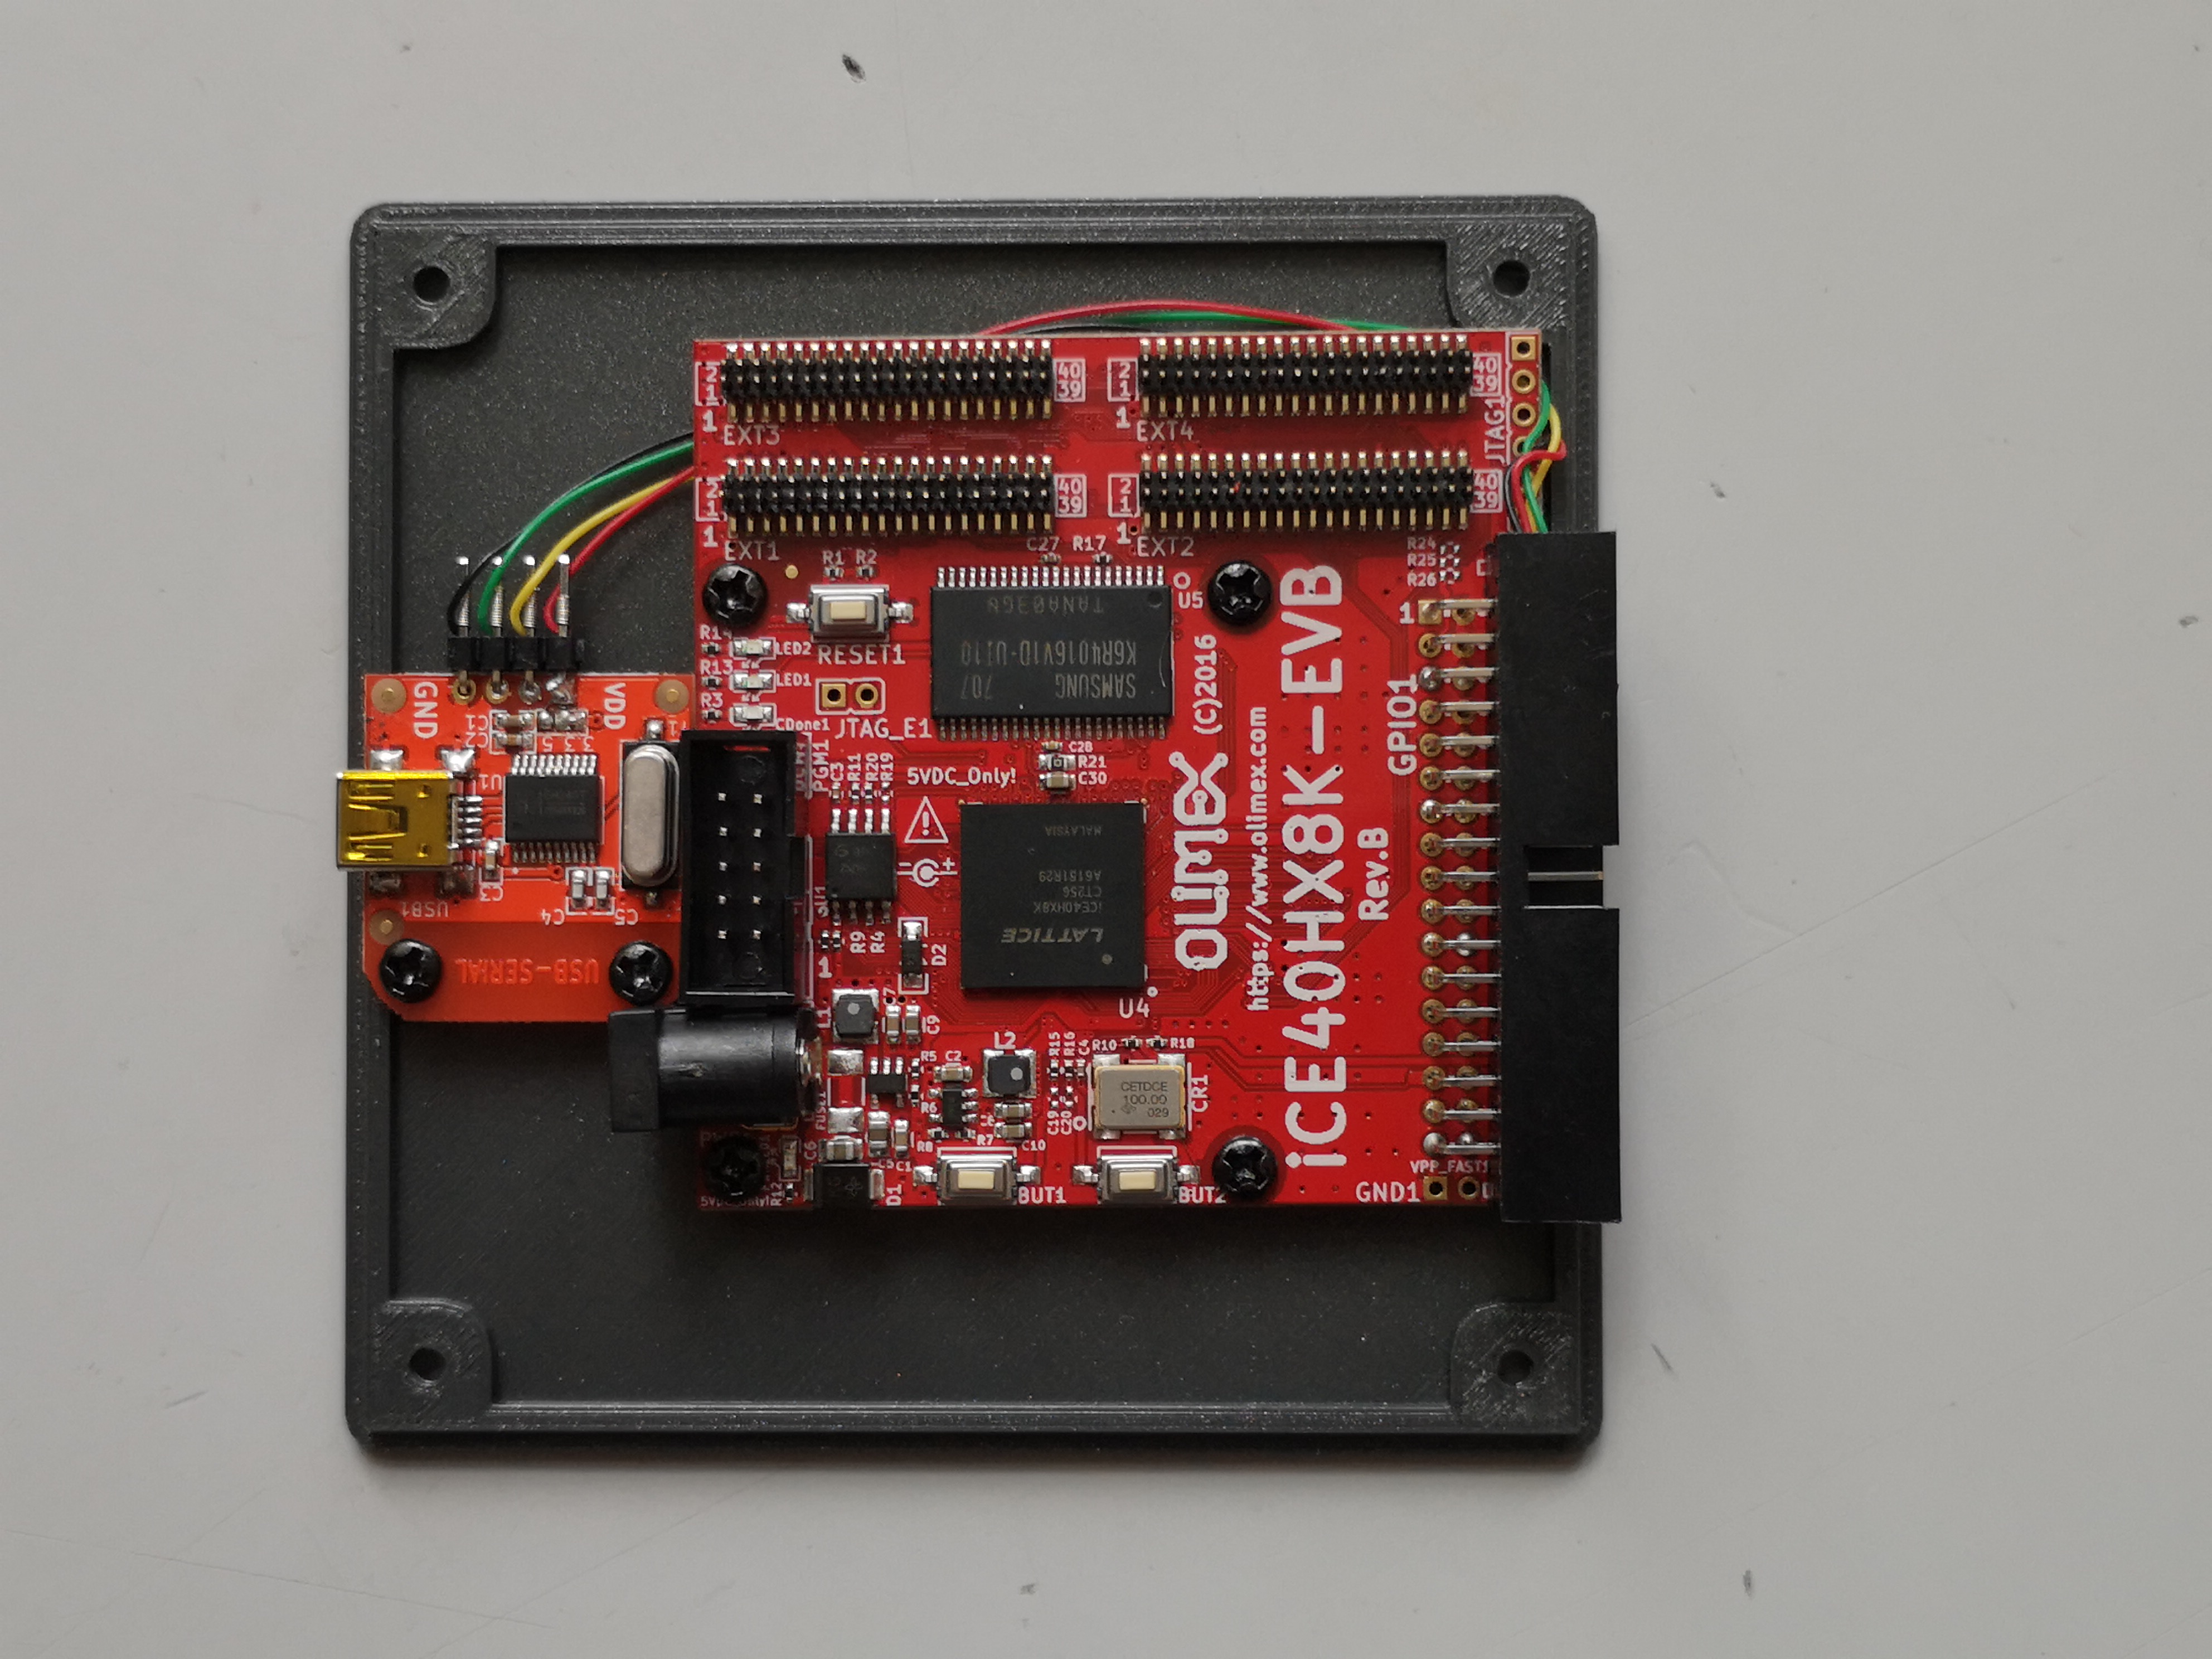
\includegraphics[width=0.7\linewidth]{MIX_inside.jpg}
	\caption{The two boards interconnected with wire wrap technique typical for computers of the 60s era}
	\label{fig:mixinside}
\end{figure}




\subsubsection{Basic unit of time}
MIX runs on iCE40HX8K-EVB clocked at \SI{23.8}{MHz}. The basic unit of time $u$ corresponds to $1u=\SI{42}{ns}$, so according to Knuth it's a relatively high priced machine.

\subsubsection{Character based I/O units U16-U20}
In our MIX implementation all character based I/O units (U16 -- U20) are connected to the USB-connector and can be accessed as serial data streams. You can connect MIX with any PC running a terminal emulator (e.g. screen for linux). The terminal should be set to 115200 baud (8N1). A conversion between ASCII and Knuths character codes is done in hardware according to Knuths specification (see TAOCP p. 128).



\subsubsection{The block based I/O unit U0}

A block based device is implemented on I/O unit 0. The device acts as a tape with 1024 blocks à 100 words. The data is stored in the SRAM chip included on the iCE40HX8K-EVB board. The speed of read and write operations is exactly $401 u$ for reading or writing one complete block of data (no \lstinline|JBUS| is needed). The data stored to unit U0 can be retrieved also after a reset (GO-Button). But on a full shutdown, when removing power supply (USB connector) data is lost.

\begin{figure}
	\centering
	\includegraphics[width=0.45\linewidth]{MIX_usb.jpg}
	\includegraphics[width=0.45\linewidth]{MIX_gpio.jpg}
	
	\caption{All character based I/O is done through a USB to serial adapter @115200 baud (8N1). MIX can be expanded through a GPIO connector placed at the rear side }
	\label{fig:mixusb}
\end{figure}



\subsubsection{MIX commands}
All commands described in TAOCP Vol. 1 are implemented (s. table \ref{tab:commands} ) with execution times corresponding to Knuth's specifications. Special care is given to the correct timings. Even the "sofisticated" commands \lstinline|SRC| and \lstinline|SLC|, which need a modulo 10 computation are executed in the defined timing of two cycles.

\begin{table}
	\centering
	\label{tab:commands}
\caption{	MIX commands}
\begin{tabular}{|l|c|c|c|}

	\hline 
	\textbf{Command} & \textbf{OP} & \textbf{Field} & \textbf{Timing} \\ 
	\hline 
 \lstinline|NOP|     & 0   & 0     & $1u$     \\
	\hline 
 \lstinline|ADD|, \lstinline|SUB|, \lstinline|MUL|, \lstinline|DIV|     & 1, 2, 3, 4   & 0:5   & $2u$, $2u$, $10u$, $12u$     \\
 	\hline 
 \lstinline|FADD|, \lstinline|FSUB|, \lstinline|FMUL|, \lstinline|FDIV|   & 1, 2, 3, 4   & 6     & $4u$, $4u$, $9u$, $11u$     \\
 	\hline 
 \lstinline|NUM|, \lstinline|CHAR|& 5   & 0, 1   & $10u$    \\
 	\hline 
 \lstinline|HLT|     & 5   & 2     & $1u$ or $\infty$?   \\
 	\hline 
 \lstinline|SLA|, \lstinline|SRA|, \lstinline|SLAX|, \lstinline|SRAX|, \lstinline|SLC|, \lstinline|SRC|& 6  & 0---5&  $2u$     \\
 	\hline 
 \lstinline|MOVE|    & 7   & F     & $(1+2F)u$\\
 	\hline 
 \lstinline|LDr|, \lstinline|LDNr|    &16---23&0:5   & $2u$     \\
 	\hline 
 \lstinline|STr|     &24---31& 0:5   & $2u$     \\
 	\hline 
 \lstinline|STJ|     & 32  & 0:2   & $2u$     \\
 	\hline 
 \lstinline|STZ|     & 33  & 0:5   & $2u$     \\
	\hline 
\lstinline|JBUS|, \lstinline|JRED|&34,38& U     & $1u$     \\
	\hline 
 \lstinline|IOC|     & 35  & U     & $1u$     \\
	\hline 
 \lstinline|IN|, \lstinline|OUT|  &36,37& U     & $(1+T)u$ \\
	\hline 
\lstinline| JMP|, \lstinline|JSJ|, \lstinline|JOV|, \lstinline|JNOV|, \lstinline|JL|, \lstinline|JE|, \lstinline|JG|, \lstinline|JGE|, \lstinline|JNE|, \lstinline|JLE|& 39  &0---9  & $1u$   \\
 	\hline 
 \lstinline|JrN|, \lstinline|JrZ|, \lstinline|JrP|, \lstinline|JrNN|, \lstinline|JrNZ|, \lstinline|JrNP|, \lstinline|JrE|, \lstinline|JrO| & 40-47& 0---7 & 	$1u$ \\
	\hline 
 \lstinline|INCr|, \lstinline|DECr|, \lstinline|ENTr|, \lstinline|ENNr|  & 48---53   &0---3     & $1u$   \\
	\hline 
 \lstinline|CMPr| & 54---63&0:5          & $2u$   \\
	\hline 
\end{tabular} 
\end{table}



The system can (easily) be extended in various ways:

\begin{enumerate}
	\item add more commands:
	\begin{itemize}
		\item logic operators: \lstinline|AND|, \lstinline|OR|, \lstinline|XOR|, \lstinline|NOT|
		\item \lstinline|JrE|,\lstinline|JrO| jump if Register r is even/odd (done)
		\item Floating point arithmetic: \lstinline|FADD|, \lstinline|FSUB|, \lstinline|FMUL|, \lstinline|FDIV| (done)
		\item Floating point compare: \lstinline|FCMP| (to do)
	\end{itemize}
	\item add more hardware:
	\begin{itemize}
		\item add leds to run the traffic light example (s. chapter \ref{traffic} of this manual)
		\item add more I/O unit
	\end{itemize}
\end{enumerate}

\subsubsection{The GO button}
MIX comes with the \textit{GO button} attached to USB-UART. So after pressing the \textit{GO button} MIX-programms can be uploaded by sending the \textit{punched cards} to USB-UART.

\subsubsection{The toast case}
MIX comes in a nice case with formfactor of a slice of toast ($\SI{10}{cm} \times \SI{10}{cm} \times \SI{2}{cm}$), so your complete MIX computer system will easily fit into your lunch box. The case can be printed with a 3D printer. Design files can be found in the directory \lstinline|build/toast| of the project site.


\section{Running programs on MIX}
\subsection{tools}
To run mixal programs on your MIX the following tools found in \lstinline|mixal/tools| 
\footnote{\href{www.gitlab.com/x653/mix-fpga}{www.gitlab.com/x653/mix-fpga}} are needed:
\begin{itemize}
	\item \lstinline|asm.py|: translates the mixal program into numeric representation (\lstinline|.mls|).
	
	\item \lstinline|mls2card.py|: translate the machine code (\lstinline|.mls|) to punchcard format. The first two cards beeing the loading routine (1.3.1.ex26) and the last card beeing the transfer card.
	
	\item \lstinline|mls2char.py|: translate to character codes, which can directly be read by MIX. (This is only necessary for the card-loading routine written on the first two punch cards).
	
	\item \lstinline|mls2bin.py|: translate the \lstinline|.mls| file to binary. This is only necessary for the GO button, which is hardcoded into fpga ROM.	
\end{itemize}

\subsection{V1: upload and run in a screen session}
Finally you can connect your PC to MIX with a USB cable and start the  terminal emulator (\lstinline|screen|):

\begin{lstlisting}[numbers=none,frame=none]
$ screen /dev/ttyUSB0 115200
\end{lstlisting}

Press the \textit{GO button} to start MIX. You should see the MIX welcome message:

\begin{lstlisting}
WELCOME TO MIX. 1U = 40NS. U16-U20 TO UART @115200 BAUD (8N1).        
\end{lstlisting}

If \lstinline|screen| does not open the terminal try with \lstinline|sudo screen|. This might happen, when the user is not allowed to acces the device \lstinline|/dev/ttyUSB0|. Check the user setting of \lstinline|/dev/ttyUSB0| and add the user to the dialout group \lstinline|sudo usermod -a -G $USER dialout|.

Within  the screen session you can upload the mixal programs written on punch cards:
\begin{lstlisting}[language=bash,numbers=none,frame=none]
<ctrl-a> : readreg p p.card
<ctrl-a> : paste p
\end{lstlisting}

\subsection{V2: Upload and run using the Makefile}
As an alterntive to \lstinline|screen| you can send jobs to MIX using a \lstinline|Makefile|. Every tested program comes in a subfolder with a corresponding \lstinline|Makefile|, which can be used to compile, upload, and run the program on MIX.

\begin{itemize}
	\item Connect MIX to USB
	\item Press the GO button
	\item run the Makefile
	\item the output is stored in a \lstinline|.out| file
\end{itemize}

\begin{lstlisting}[numbers=none,frame=none]
$ make clean
$ make
\end{lstlisting}


\subsection{Verify}

MIX has been verified with the following programms. The numbering correspond to the sections in TAOCP.
\begin{itemize}	
\item \lstinline|1.3.1ex26| card-loading routine
\item \lstinline|1.3.2P| table of primes
\item \lstinline|1.3.2E| easter dates
\item \lstinline|1.3.2.ex13| cryptanalyst problem (classified)
\item \lstinline|1.3.2.ex16| sum of harmonic series
\item \lstinline|1.3.2.ex20| josephus problem
\item \lstinline|1.3.2.ex22| traffic signal problem (driving real LEDs)
\item \lstinline|1.3.3A| multiply permutations in cycle form
\item \lstinline|1.4.2|  character input routine
\item \lstinline|1.4.3|  trace routine (uses tape U0)
\item \lstinline|2.2.5elevator| elevator simulation (with added in-/output)
\item \lstinline|mixaload| A load and go assembler by James L. Peterson from "Computer Organization and Assembly Language Programming" \footnote{\href{http://www.jklp.org/profession/books/mix/index.html}{http://www.jklp.org/profession/books/mix/index.html}}

\end{itemize}

\section{Example program 1.3.2P}

We will run programm \lstinline|P| of chapter 1.3.2 TAOCP (p. 148) on MIX. Programm \lstinline|P| computes the first 500 primes and outputs them in a table on the line printer U18.

\subsection{Prepare the input}
\subsubsection{p.mixal}
The mixal program can be found in \lstinline|mixal/1.3.2P/p.mixal|:

\begin{lstlisting}[numbers=none,frame=none]
$ cd mixal/1.3.2P
$ cat p.mixal
\end{lstlisting}

\lstinputlisting{../mixal/1.3.2P/p.mixal}

\subsubsection{p.mls}
First we translate the mixal programm to binary code. This is done with the translator \lstinline|tools/asm.py|.

\begin{lstlisting}[numbers=none,frame=none]
$ ../tools/asm.py p.mixal
$ cat p.mls
\end{lstlisting}

\lstinputlisting{../mixal/1.3.2P/p.mls}

\subsubsection{p.card}
Next we must write the binary code onto punched cards. This can be done with the python script \lstinline|mixal/tools/mls2card.py|.
The python scripts reads the listing file \lstinline|p.mls|, extracts the numeric codes and writes them in the file \lstinline|p.card| in puncher card format.

Every line of \lstinline|p.card| holds 80 chars of a card. The first two cards contain the card loading routine discussed in exercise 26 in chapter 1.3.1 of TAOCP. The last card is the so called transfer card, which tells the bootloader to start execution at memory location 3000.

\begin{lstlisting}[numbers=none,frame=none]
$ ../tools/mls2card.py p.mls
$ cat p.card
\end{lstlisting}

\lstinputlisting{../mixal/1.3.2P/p.card}

\subsubsection{go!}
Power MIX with USB cable connected to your computer.
Start a screen session with 115200 baud (8N1)
\begin{lstlisting}[numbers=none,frame=none]
screen /dev/ttyUSB0 115200
\end{lstlisting}

Press the \textit{GO button} on MIX. You should see the welcome message on your terminal:
\begin{lstlisting}
WELCOME TO MIX. 1U = 40NS. U19 @115200 BAUD (8N1).                    
\end{lstlisting}

\subsubsection{input the cards to U16}
You can now send the punched cards to MIX within the screen terminal session.
Read cards into a screen-buffer (called p) and send the buffer to MIX.

\begin{lstlisting}[numbers=none,frame=none]
<in screen terminal> Ctr-a : readreg p p.card <enter>
<in screen terminal> Ctrl-a : paste p <enter>
\end{lstlisting}

After a short amount of time MIX spits out the following table to the printer U18. Notice that output to U18 have 120 characters per line, while output to the terminal U19 is only 70 chars wide.

\lstinputlisting{../mixal/1.3.2P/p.out}

\subsection{Congratulation}
You have run your first program on a \textit{real} MIX.

\subsection{Using Makefile}
With the included \lstinline|Makefile| the above described steps can be done in one pass:

\begin{itemize}
	\item Connect MIX to USB
	\item Press the GO button
	\item run the Makefile: \lstinline|$ make|
	\item the output is stored in \lstinline|p.out| file
\end{itemize}


\section{Build your own MIX and/or modify the fpga design}

The project runs on iCE40HX8K-EVB fpga from Olimex Ltd. The whole project uses only FOSS soft- and hardware. With little modifications it should run on any fpga board available out in the wild.

\subsection{Requirement}
\begin{enumerate}
	\item 
	fpga board (iCE40HX8K-EVB)
	\item programmer device (Olimexino 32u4) with idc10 cable (cable-IDC10)
	\item USB-UART-board (BB-CH340T).  
	\item fpga toolchain. The project was developed with \lstinline|apio| \footnote{\href{github.com/FPGAwars/apio}{github.com/FPGAwars/apio}}, a software suite based on project icestorm\footnote{\href{www.clifford.at/icestorm}{www.clifford.at/icestorm}} from Clifford Wolf.
\end{enumerate}

Consider to buy at Olimex Ltd. \footnote{\href{www.olimex.com}{www.olimex.com}}, the company with the highest number of registered OSHW-projects. Install the tools with:

\begin{lstlisting}[numbers=none,frame=none]
$ sudo pip install -U apio
$ apio install ice40
$ apio install iverilog
$ apio install scons
$ apio install yosys
$ sudo apt install gtkwave
$ cd build/iceprogduino
$ make
$ sudo make install
$ sudo apt install screen
\end{lstlisting}

\subsection{FPGA iCE40HX8K-EVB}

Build the project and upload the circuit design to the fpga:

\begin{enumerate}
	\item cd into the directory \lstinline|rtl| and build the project

	\begin{lstlisting}[numbers=none,frame=none]
	$ cd rtl
	$ apio clean
	$ apio build -v
	\end{lstlisting}
	
	\item Connect the fpga board with olimexino-32u4 programmer to upload the bitstream file. Use two USB cables to power both boards as shown in fig. \ref{fig:flash}.
	
	\item Upload the bitstream file to fpga board.
	
	\begin{lstlisting}[numbers=none,frame=none]
	$ cd build/rtl
	$ apio clean
	$ apio build -v
	$ apio upload
	\end{lstlisting}
\end{enumerate}



\begin{figure}
	\centering
	\includegraphics[width=0.6\linewidth]{MIX_flash.jpg}
	\caption{Connect programmer Olimexino-32u4 with fpga board iCE40HX8K-EVB}
	\label{fig:flash}
\end{figure}




\subsection{The USB-serial adapter}
The serial adapter BB-CH340T is used to:
\begin{enumerate}
	\item  Power MIX with 5Volt from USB cable
	\item  Serial communication to MIX over I/O Unit 16-20.
\end{enumerate}

To use USB-Serial adapter as power source we must do a little modification on the board according to Fig. \ref{fig:detail}:
\begin{enumerate}
	\item  cut with a cutter knife the connection marked in GREEN, and
	\item  solder a bridge BLACK between the right most terminal (VDD) and the 5V pad.
\end{enumerate}

This will ensure that the right most terminal connector (red cable) get's 5Volt form USB, which will be used to power the fpga board. But the UART signals (green and yellow cables) are still leveled to 3.3V, which corresponds to the in-/output signal level of fpga-connector GPIO1.


\begin{figure}
	\centering
	\includegraphics[width=0.5\linewidth]{detail.png}
	\caption{Cut the pcb track (GREEN) and solder a bridge from 5V pad to the right most connector pin.}
	\label{fig:detail}
\end{figure}

The 4 wires are connected to the GPIO connector on the right side of iCE40HX8K-EVB according to the following table. Compare with schematic in the appendix  \ref{sec:schematic}.

\begin{table}[H]
	\centering	
	\begin{tabular}{|c|c|c|}
		\hline 
		color & USB-serial & GPIO (ICE40HX8K-EVB) \\ 
		\hline 
		black & GND & 2 \\ 
		\hline 
		green & RX & 7 \\ 
		\hline 
		yellow & TX & 5 \\ 
		\hline 
		red & VDD & 1 \\ 
		\hline 
	\end{tabular} 
\end{table}


\subsection{The Go button}
We will implement the code needed by the go button proposed in  exercise 26 in chapter 1.3.1 of TAOCP (see p. 510).

\subsubsection{prepare the software}
The mixal program can be found in \lstinline|go/go.mixal|. It starts at location 4000 (which is implemented in fpga but not used by MIX). The programm spits out the welcome message. The JMP instruction at memory cell 4095 will jmp to location 0 storing a +0000 in the J-Register, because beeing a binary version with 12 bit programmcounter the next execution address without the jmp instruction would equally yield 4095 + 1 = 0000.


\lstinputlisting{../build/go/go.mixal}

First we translate the mixal programm to binary code with \lstinline|mixal/tools/asm.py|.

\begin{lstlisting}[numbers=none,frame=none]
$ cd build/go
$ ../../mixal/tools/asm.py go.mixal
$ cat go.mls
\end{lstlisting}

\lstinputlisting{../build/go/go.mls}

Next we must translate the binary code into a binary format readable by the fpga toolchain. This can be done with the python script \lstinline|mixal/tools/mls2bin.py|.

\begin{lstlisting}[numbers=none,frame=none]
$ ../../mixal/tools/mls2bin.py go.mls
$ cat go.bin
\end{lstlisting}



The python scripts reads the listing file \lstinline|go.mls|, extracts the code and writes it in the file \lstinline|go.bin|.

Inspect the binary file `go.bin`


\lstinputlisting[firstnumber=4090,linerange=4090-4096]{../build/go/go.bin}


The output contain the program code expressed as binary numbers. These binary numbers can be flashed to the iCE40HX8K-EVB board, so it will be stored permanently in the MIX computer. At every reset (press \textit{Go button}) the code will be executed. The first 4000 zero lines translate to NOP instructions. At the end you find the sequence IN(16),JBUS,JMP...



\subsection{build and flash to iCE40HX8K-EVB}

\begin{itemize}
	\item Copy the binary file \lstinline|go.bin| into the directory \lstinline|rtl|, where the fpga description files are.
	\item Rebuild the fpga project and upload. An \lstinline|apio clean| is needed, because otherwise the preloaded memory will not be updated.	
\end{itemize}

\begin{lstlisting}[numbers=none,frame=none]
$ cp go.bin ../../rtl/go.bin
$ apio clean
$ apio build -v
$ apio upload
\end{lstlisting}

\textbf{Tipp:} change the welcome message to ensure the new rom file has been uploaded.

\subsection{print toast case with a 3D printer}
In the subfolder \lstinline|build/toast| you find printing files for the case. The case consists of three parts:

\begin{itemize}
\item \lstinline|bottom.blend|: the bottom part of the case
\item \lstinline|top.blend|: top part of case
\item \lstinline|go.blend|: go bottom
\end{itemize}

\begin{figure}
	\centering
	\includegraphics[width=0.6\linewidth]{MIX_real.jpg}
	\caption{MIX fits in nice toast like case}
	\label{fig:toast}
\end{figure}



\section{Example program 1.3.2.ex20T}
\label{traffic}
We will run programm \lstinline|T| of exercise 20 in chapter 1.3.2 TAOCP (p. 161) on MIX. Programm \lstinline|T| controls the traffic signal at corner of Del Mare Boulevard and Berkeley Avenue. This project will connect LEDs directly to the register rX and a push button to the  Overflow toggle. This will be done extending the fpga design and routing the appropriate signals to the GPIO connector at the back of MIX.

\begin{figure}
	\centering
	\includegraphics[width=0.7\linewidth]{MIX_traffic}
	\caption{Connect LEDs and push button over the GPIO connector directly to register rX to control the traffic light}
	\label{fig:mixtraffic}
\end{figure}


\subsection{Extending the fpga desing}

Make a copy of the folder \lstinline|rtl| and cd into it.

\begin{lstlisting}[numbers=none,frame=none]
$ cd build
$ cp -r rtl rtl_traffic_light
$ cd rtl_traffic_light
\end{lstlisting}


\subsubsection{mix.pcf}

Find the following lines in the physical constraint file \lstinline|mix.pcf| and uncomment to get access to the GPIO pins 9-19.

\lstinputlisting[language=verilog,firstnumber=15,linerange=15-25]{../build/rtl/mix.pcf}

\subsubsection{mix.v}

To connect the Register rX with the traffic signals: find the following lines (28--38 and 47--56) in \lstinline|mix.v| and uncomment:

\lstinputlisting[language=verilog,firstnumber=20,linerange=20-56]{../build/rtl/mix.v}

Control the overflow toggle with the button by uncommenting line 239 in the code snippet:

\lstinputlisting[language=verilog,firstnumber=237,linerange=237-245]{../build/rtl/mix.v}

\subsection{rebuild and flash to iCE40HX8K-EVB}

Rebuild the fpga project and upload.

\begin{lstlisting}[numbers=none,frame=none]
$ apio clean
$ apio upload -v
\end{lstlisting}

\textbf{Tipp}: change the welcome message to ensure the new rom file has been uploaded.

\subsection{add leds and button to GPIO}
Connect leds and button (don't forget resistors) to the appropriate GPIO connectors as described in the \lstinline|mix.pcf| file. For simplicity only one LED is shown below:

\begin{figure}[H]
	\centering
	\input{schaltung_gpio_led.cir}
	\caption{connect LED and button to GPIO connector}
	\label{fig:leds}
\end{figure}


\textbf{Attention}: gpio pins 1,2,5 and 7 are already used by the internal USB-serial converter.


\subsection{t.mixal}
Compile and write \lstinline|mixal/1.3.2.ex20/t.mixal| to puching card format. Start MIX by pressing the \textit{go button}. Upload \lstinline|t.card| to MIX and see the traffic signals blinking.


\section{Service}
In case you encounter an issue with MIX:
\begin{itemize}
	\item don't panic
	\item plese send an email to the author\footnote{mi.schroeder@netcologne.de} with a precise description of the problem.
\end{itemize}

\section{License}

\subsection{mix-fpga}
The project as a whole is licensed under the GPL 3 and can be found at \href{www.gitlab.com/x653/mix-fpga}{www.gitlab.com/x653/mix-fpga}.
\subsection{manual}
\doclicenseThis

\newpage

\appendix

\section{Schematic iCE40HX8K-EVB}
\label{sec:schematic}
\includegraphics[angle=90,scale=0.8]{iCE40HX8K-EVB.pdf}

\section{Schematic BB-CH340T}
\label{sec:schematic}
\includegraphics[scale=0.2]{bb_ch340t.png}


\end{document}
